\documentclass[11pt]{article}
\usepackage[title]{appendix}
\usepackage{amsmath,amssymb,amsthm}
\usepackage{enumitem}
\usepackage[left=1in,right=1in,top=1in,bottom=1in]{geometry}
\usepackage{tikz}
\usetikzlibrary{cd,calc,intersections,decorations.pathmorphing}
\usepackage{xcolor}
\usepackage{sectsty,wrapfig}
\usepackage{hyperref}
\allowdisplaybreaks

\newtheorem{thm}{Theorem}[section]
\newtheorem{prp}[thm]{Proposition}
\newtheorem{lmm}[thm]{Lemma}
\newtheorem{crl}[thm]{Corollary}
\newtheorem{ques}[thm]{Question}
\newtheorem{fact}[thm]{Fact}

\theoremstyle{definition}
\newtheorem{dfn}[thm]{Definition}
\newtheorem{eg}[thm]{Example}

\theoremstyle{remark}
\newtheorem{rmk}[thm]{Remark}

\def\wt#1{\widetilde{#1}}
\def\ov#1{\overline{#1}}
\def\mr#1{{\mathring{#1}}}

\def\sgray{{\textnormal{gray}}}
\def\sred{{\textnormal{red}}}
\def\syellow{{\textnormal{yellow}}}
\def\sorange{{\textnormal{orange}}}
\def\sblue{{\textnormal{blue}}}


\def\Z{\mathbb{Z}}
\def\C{\mathbb{C}}
\def\P{\mathbb{P}}
\def\R{\mathbb{R}}
\def\Q{\mathbb{Q}}
\def\D{\mathbb{D}}
\def\fc{\mathfrak{c}}
\def\ff{\mathfrak{f}}
\def\fs{\mathfrak{s}}
\def\M{\mathfrak{M}}
\def\S{\mathfrak{S}}
\def\fT{\mathfrak{T}}
\def\cA{\mathcal{A}}
\def\cD{\mathcal{D}}
\def\cG{\mathcal{G}}
\def\cI{\mathcal{I}}
\def\cM{\mathcal{M}}
\def\cT{\mathcal{T}}
\def\cN{\mathcal{N}}
\def\cP{\mathcal{P}}
\def\cS{\mathcal{S}}
\def\cU{\mathcal{U}}
\def\rI{{\mathring{I}}}

\def\cmt#1{\textcolor{red}{(#1)}}
\def\tn#1{\textnormal{#1}}
\def\pr{{\textnormal{pr}}}


\begin{document}

\setlength{\parskip}{\baselineskip}
\setlength{\parindent}{0cm}

\section{Introduction}

.....(introduction)

{\bf Define the kind of bundle we work with in this paper:}
Given a smooth homology sphere $M$, define a {\it framed $(M,\infty)$-bundle} $(\pi:E\to B,\sigma, \tau, F)$ (abbreviate all these to $\pi$) to be a smooth fiber bundle $\pi:E\to B$ with fiber $M$, with a smooth section $\sigma$, a trivialization $\tau$ of the bundle near $\sigma$, and a smooth vertical framing $F$ of $\pi$ ``standard'' near $\sigma$. 

{\bf Define the bracket operation, $\pi_1,\pi_2\to[\pi_1,\pi_2]$ on such bundles, in an intuitively clear but not necessarily rigorous way.}

{\bf Define cobracket and coproduct on graph cohomology (everything is over $\Q$):}
\begin{itemize}
\item First, define the graph complex $\cG'$---the $\Q$-vector space spanned by (with correct orientation definition, omitted here) connected graphs containing either a univalent vertex or a simple loop (an edge starting and ending at the same vertex). 
The coboundary operation $\delta$ is given by contracting an edge. 
In $\delta$ and all the operations on graphs below, whenever a graph not in $\cG'$ appears (a graph that has a univalent vertex or simple loop), we set it to 0. 
\item Taking the homology of $\cG'$ with respect to $\delta$, denote by $H^*{\cG'}$. 

\item Define the cobracket operation to be the linear map
\begin{align}\label{graphcobracket_eqn}
\Delta_{[,]}: \cG'&\longrightarrow\cG'\otimes\cG'\nonumber\\
\Gamma&\longrightarrow \sum_{\Gamma'\le\Gamma}\big(\Gamma'\otimes\Gamma/\Gamma'+(-1)^{..}\Gamma/\Gamma'\otimes\Gamma'\big), 
\end{align}
where $\Gamma'$ ranges through all full subgraphs of $\Gamma$ that is connected, with no univalent vertex or simple loop.
\item Check that $\Delta_{[,]}$ commutes with $\delta$ and $\delta\otimes\tn{id}\pm\tn{id}\otimes\delta$, so it descends to 
$$\Delta_{[,]}: H^*{\cG'}\longrightarrow H^*(\cG'\otimes\cG')\approx H^*{\cG'}\otimes H^*{\cG'}.$$

\item Finally we also define the coproduct operation on $\cG'$ (this makes more sense for disconnected graphs but w=for connected graphs it is extra simple):  
\begin{align*}
\Delta_{\cdot}: \cG'&\longrightarrow \cG'\otimes\cG'\\
\Gamma&\longrightarrow \Gamma\otimes \tn{(the empty graph)} + \tn{(the empty graph)}\otimes\Gamma.
\end{align*}

\end{itemize}

{\bf Brief introduction to Kontsevich's characteristic classes.}
Given a framed $(M,\infty)$-bundle $\pi:E\to B$ as above, denote by  
$$K_\pi: H^*(\cG')\longrightarrow H^*(B)$$
Kontsevich's characteristic classes of $\pi$. 


\begin{thm}\label{formula_thm}
Suppose $d\ge3$. 
For $i=1,2$, suppose $M_i$ is a $d$-dimensional smooth homology sphere and 
suppose $\pi_i: E_i\to B_i$ is a framed $(M,\infty)$-bundle. 
(Now, $[\pi_1,\pi_2]: E\to S^d\times B_1\times B_2$ is the bracket bundle.)
Then, for all $\eta\in H^*\cG'$, 
\begin{align*}
K_{[\pi_1,\pi_2]}(\eta)=
\tn{PD}_{S^d}[S^d]\otimes
(K_{\pi_1}\otimes K_{\pi_2})(\Delta_{[,]}(\eta))
+\tn{PD}_{S^d}[pt]\otimes
(K_{\pi_1}\otimes K_{\pi_2})(\Delta_\cdot(\eta)).
\end{align*}
(Both LHS and RHS lives in 
$$H^*(S^d\times B_1\times B_2)\approx H^*(S^d)\otimes H^*(B_1)\otimes H^*(B_2).$$
$\tn{PD}_{S^d}$ means Poincar\'e dual on $S^d$; $[S^d]$ stands for the fundamental class of $S^d$ and $[pt]$ stands for the point class of $S^d$.)
\end{thm}


......(Then talk about the $(d+1)$-fold loop space structure on $\tn{BDiff}^{\tn{fr}}_\partial(D^d)$ and the theorem/corollary that it doesn't extend.)

(Below is an outline of the proof of Theorem \ref{formula_thm}.
Throughout, $\pi_1,\pi_2$ are given and fixed. 
)

\subsection{Notation}

Given a graph $G$, we denote by $V(G)$ its vertex set and $E(G)$ its edge set. 

\section{Conftilde}\label{conftilde_sec}

Construct the big configuration space $\widetilde{C}_A$. 
Show that it is a smooth manifold with boundary and corners. 
(These are mostly already written in the file ``conftilde'' I sent a while ago.)

What we need are the following: 

\begin{itemize}
\item $\widetilde{C}_A$ is a smooth manifold with boundary and corners; 
\item each $S_T$ is a stratum of $\widetilde{C}_A$; 
\item $\overline{S}_T=\bigsqcup_{T'}S_{T'}$, where the disjoint union is taken over all $A$-labeled trees $T'$ such that $T$ can be obtained from $T'$ by contracting some edges. 

\end{itemize}

Here is a schematic picture of $\wt{C}_A$ (the marked points are not drawn; the actual stratification structure of $\wt{C}_A$ is more complicated than what is shown in the picture): 

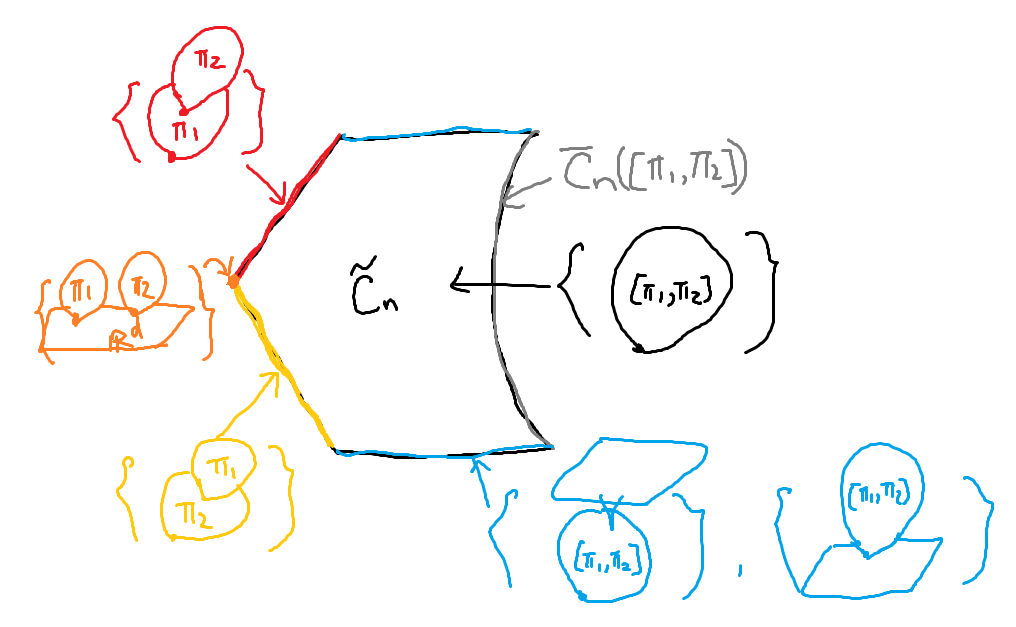
\includegraphics[scale=0.7]{conftilde.png}

The boundary of $\wt{C}_A$ consists of the following parts: 
\begin{itemize}
\item the gray part, denoted by $\ov{S}_\sgray$, is $\ov{C}_A([\pi_1,\pi_2])$; its interior, denoted by $S_\sgray$, is $C_A([\pi_1,\pi_2])$; 
\item ${S}_\sblue:=\bigcup_{T\in\cT_\sblue}S_T$, where $\cT_\sblue$ is the set of all $A$-labeled trees whose shape and space labels are like
$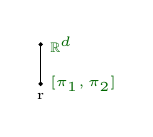
\begin{tikzpicture}
\node [below] at (0,0) {\tiny{r}};  
\node [right, black!60!green] at (0,0) {\tiny{$[\pi_1,\pi_2]$}};
\node [right, black!60!green] at (0,0.5) {\tiny{$\R^d$}};
\draw [fill] (0,0) circle [radius=0.02];
\draw [fill] (0,0.5) circle [radius=0.02];
\draw (0,0) -- (0,0.5);
\end{tikzpicture}$ or 
$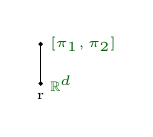
\begin{tikzpicture}
\node [below] at (0,0) {\tiny{r}};  
\node [right, black!60!green] at (0,0) {\tiny{$\R^d$}};
\node [right, black!60!green] at (0,0.5) {\tiny{$[\pi_1,\pi_2]$}};
\draw [fill] (0,0) circle [radius=0.02];
\draw [fill] (0,0.5) circle [radius=0.02];
\draw (0,0) -- (0,0.5);
\end{tikzpicture}$;
and let $\ov{S}_\sblue$ be the closure of $S_\sblue$;
\item ${S}_\sred:=\bigcup_{T\in\cT_\sred}S_T$, where $\cT_\sred$ is the set of all $A$-labeled trees with the following shape and space labels: 
$\begin{tikzpicture}
\node [below] at (0,0) {\tiny{r}};  
\node [right, black!60!green] at (0,0) {\tiny{$\pi_1$}};
\node [right, black!60!green] at (0,0.5) {\tiny{$\pi_2$}};
\draw [fill] (0,0) circle [radius=0.02];
\draw [fill] (0,0.5) circle [radius=0.02];
\draw (0,0) -- (0,0.5);
\end{tikzpicture}$;
and let $\ov{S}_\sred$ be the closure of $S_\sred$;
\item ${S}_\syellow:=\bigcup_{T\in\cT_\syellow}S_T$, where $\cT_\syellow$ is the set of all $A$-labeled trees with the following shape and space labels: 
$\begin{tikzpicture}
\node [below] at (0,0) {\tiny{r}};  
\node [right, black!60!green] at (0,0) {\tiny{$\pi_2$}};
\node [right, black!60!green] at (0,0.5) {\tiny{$\pi_1$}};
\draw [fill] (0,0) circle [radius=0.02];
\draw [fill] (0,0.5) circle [radius=0.02];
\draw (0,0) -- (0,0.5);
\end{tikzpicture}$;
and let $\ov{S}_\syellow$ be the closure of $S_\syellow$; 
\end{itemize}

We also define
${S}_\sorange:=\bigcup_{T\in\cT_\sorange}S_T$, where $\cT_\sorange$ is the set of all $A$-labeled trees with the following shape and space labels: 
$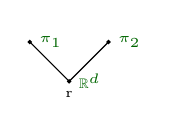
\begin{tikzpicture}
\node [below] at (0,0) {\tiny{r}};  
\node [right, black!60!green] at (0,0) {\tiny{$\R^d$}};
\node [right, black!60!green] at (-0.5,0.5) {\tiny{$\pi_1$}};
\node [right, black!60!green] at (0.5,0.5) {\tiny{$\pi_2$}};
\draw [fill] (0,0) circle [radius=0.02];
\draw [fill] (-0.5,0.5) circle [radius=0.02];
\draw [fill] (0.5,0.5) circle [radius=0.02];
\draw (-0.5,0.5) -- (0,0) -- (0.5,0.5);
\end{tikzpicture}$;
and let $\ov{S}_\sorange$ be the closure of $S_\sorange$. Then, $\ov{S}_\sorange=\ov{S}_\sred\cap\ov{S}_\syellow$. 

We define $\ov{C}^*_A=\ov{S}_\sred\cup\ov{S}_\syellow$.

% note that 
%${S}_T$ is a 1-parameter family of $\partial \ov{C}_n([\pi_1,\pi_2])$---its interior is diffeomorphic to 
%$$\partial \ov{C}_n([\pi_1,\pi_2])\times (0,1);$$

\section{Propagators}\label{propagator_sec}

Before starting the discussion on propagators, we first define another notion of ``forgetful map''. 

Given finite sets $A$ (``set of point labels'') and $B$ (``set of space labels''), recall the definition of an $(A,B)$-labeled tree in ...\textcolor{red}{(change the definition in conftilde to allow arbitrary space labels!)}

In all the cases we care about, the elements of $B$ will be $(M,\infty)$-bundles for some $d$-dimensional manifold $M$. 

In this paper we only consider cases when $|B|\le2$. 
Define 
$$\wt{C}_{A}(B)=\begin{cases}
\ov{C}_A(\R^d)\tn{ if }B=\emptyset,\\
\ov{C}_A(\pi)\tn{ if }B=\{\pi\}\tn{ for some }(M,\infty)-\tn{bundle }\pi,\\
\wt{C}_A\backslash\ov{S}_\sgray\tn{ if }B=\{\pi_1,\pi_2\}\tn{ for some }(M_1,\infty)\tn{-bundle }\pi_1\tn{ and some }(M_2,\infty)\tn{-bundle }\pi_2.
\end{cases}$$
Then, the strata of $\wt{C}_A(B)$ are in 1-to-1 correspondence with $(A,B)$-labeled trees. 
Given such a stratum $S$, we denote by $\cT_S$ the tree corresponding to it and given such a tree $T$ we denote by $\cS_T$ the stratum corresponding to it. \footnote{\cmt{$\cT$ was used previously in conftilde; maybe change it to $\fT$ there.}}
The condition $\cS_{T'}\subset\ov{\cS}_T$ is equivalent to that $T$ can be obtained from $T'$ by contracting some edges. In this case, the set of edges to be contracted to get from $T'$ to $T$ is unique and we denote by $\fc_{T',T}:V(T')\to V(T)$ the map on the vertices induced by the contraction. 
Also define 
$\mathfrak{i}_{T',T}:V(T)\to V(T')$
mapping $v$ to the lowest vertex in $\fc_{T',T}^{-1}(v)$. 
The following lemma is immediate: 

\begin{lmm}\label{treecontr1_lmm}
Let $T',T$ be $(A,B)$-labeled trees such that $T$ can be obtained from $T'$ by contracting some edges. 
Then, for every $v\in V(T)$, $lp(\ge v)=lp(\ge \mathfrak{i}_{T',T}(v))$. 
\end{lmm}


\textcolor{red}{Maybe move the above to an earlier section devoted to combinatorics.}


For the rest of this section we only consider the case $A=\{1,2\}$. Let $B$ be a finite set such that every element of $B$ is an $(M,\infty)$-bundles for some $d$-dimensional manifold $M$, and $|B|\le2$. 
\begin{dfn}%\footnote{\textcolor{red}{not great; try to improve the exposition later}}
Let $T$ be a $(\{1,2\},B)$-labeled tree,
\footnote{The definition obviously extends to the case of an arbitrary number of marked points and forgetting to an arbitrary subset of marked points, but we only need this simple 2 point case here.}
then $\cS_T\approx\prod_{v\in V(T)}C_{lp(v)\cup cld(v)}(ls(v))$ is a stratum in $\wt{C}_{\{1,2\}}(B)$.
Define $\nu_{T}\in V(T)$ to be the vertex such that $\{1,2\}\subset lp(\ge \nu_{T})$ and for all $v>\nu_{T}$, $\{1,2\}\not\subset lp(\ge v)$.\footnote{\cmt{In this paper $\subset$ means subset or equal. Specify this somewhere early.}}
Define $\fs_{T}:=ls(\nu_T)$. \footnote{\cmt{Actually, maybe use $\mathfrak{p},\fs$ instead of fp,fs?}}
\begin{itemize}
\item Define 
$$\hat{f}_{T}:\cS_T\longrightarrow {C}_{2}(\fs_{T}),\qquad \hat{f}_{T}\big((c_v)_{v\in V(T)}\big)=c'_{\nu_{T}},$$
where $c'_{\nu_{T}}\in C_{2}(\fs_{T}))$ is obtained from $c_{\nu_{T}}$ by forgetting all the points except for two: $f_{\nu_{T}}(1)$ and $f_{\nu_{T}}(2)$. \textcolor{red}{($f_v$ is defined in conftilde, at the beginning of Section 3.3.)}

\item Suppose $T'$ is a $(\{1,2\},B)$-labeled tree such that $T$ can be obtained from $T'$ by contracting some edges. 
Abusing notation, we denote the subtree of $T'$ spanned by vertices in $\fc_{T',T}^{-1}(\nu_T)$ still by $\fc_{T',T}^{-1}(\nu_T)$.
Define $G_{T',T}$ to be the tree obtained from $\fc_{T',T}^{-1}(\nu_T)$ by ``stabilization with respect to $\{1,2\}$ and $\fs_T$'', namely: let $V'\subset V(\fc_{T',T}^{-1}(\nu_T))$ (``set of unstable vertices'') consist of vertices $v$ such that $\tn{lsset}(ls(v))\cap\tn{lsset}(ls(\nu)_T)=\emptyset$ and $|lp(\ge v)\cap\{1,2\}|<2$; 
define $G_{T',T}$ to be obtained from $\fc_{T',T}^{-1}(\nu_T)$ by: for every vertex $v\in V'$, contracting the edge just below $v$. 
Then, $\cS_{G_{T',T}}$ is a stratum of $\ov{C}_2(\fs_T)$. 
Define
$$\hat{f}_T:\cS_{T'}\longrightarrow \cS_{G_{T',T}}\subset\ov{C}_2(\fs_T),\qquad \hat{f}_T\big((c_v)_{v\in V(T')}\big)=(c'_{v})_{v\in V(G_{T',T})},$$
where each $c'_{v}\in C_2(ls(v))$ is as follows: 
let $v'\in V(\fc_{T',T}^{-1}(\nu_T))\subset V(T')$ be the lowest vertex contracted to $v$, then $c'_{v}$ is obtained from $c_{v'}$ by forgetting all points except for two: $f_{v'}(1)$ and $f_{v'}(2)$. 
\item We have therefore defined a map 
$$\hat{f}_T:\ov{\cS}_T\longrightarrow\ov{C}_2(\fs_T).$$
It is easy to verify that $\hat{f}_T$ is smooth using the charts we constructed in Section \textcolor{red}{(conftilde section)}. 
\end{itemize}
\end{dfn}

\textcolor{red}{Maybe introduce more notation when talking about the combinatorics of $A$-labeled trees, e.g., a pre-stable tree and how to get from a pre-stable tree to a stabel tree by contraction.?}

Note that if $G_{T',T}$ has only one vertex, then $\hat{f}_{T'}=\hat{f}_{T}|_{\ov\cS_{T'}}$. Otherwise, this is not the case. 

\begin{eg}[$|B|=2$, in $\wt{C}_2$]
$T=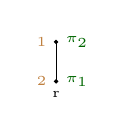
\begin{tikzpicture}
\node [below] at (0,0) {\tiny{r}};  
\node [right, black!60!green] at (0,0) {\tiny{$\pi_1$}};
\node [left, brown] at (0,0) {\tiny{2}};
\node [right, black!60!green] at (0,0.5) {\tiny{$\pi_2$}};
\node [left, brown] at (0,0.5) {\tiny{1}};
\draw [fill] (0,0) circle [radius=0.02];
\draw [fill] (0,0.5) circle [radius=0.02];
\draw (0,0) -- (0,0.5);
\end{tikzpicture}$, 
$T'=\begin{tikzpicture}
\node [below] at (0,0) {\tiny{r}};  
\node [right, black!60!green] at (0,0) {\tiny{$\pi_1$}};
\node [left, brown] at (0,0.5) {\tiny{2}};
\node [left, brown] at (0,1) {\tiny{1}};
\node [right, black!60!green] at (0,1) {\tiny{$\pi_2$}};
\draw [fill] (0,0) circle [radius=0.02];
\draw [fill] (0,0.5) circle [radius=0.02];
\draw [fill] (0,1) circle [radius=0.02];
\draw (0,0) -- (0,0.5) -- (0,1);
\end{tikzpicture}$ 
(so $\cS_{T'}\subset\ov{\cS}_T$), 

$\hat{f}_T($
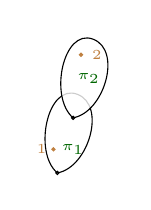
\begin{tikzpicture}%[inner sep=0pt]
%%\draw [name path=pi1] (0,0) to [out=10,in=-20] coordinate[pos=0.5](x) (0.25,1) to [out=160,in=140] coordinate[pos=0.3](y) (0,0) node(z) {}; 
%\path [name path=pi1] (0,0) to [out=10,in=-20] (0.25,1) to [out=160,in=140] (0,0) node(o) {}; 
%\draw (o) circle[fill, radius=0.01];
%\draw [name path=pi2] (0.2,0.7) coordinate(o2) to [out=10,in=-20] ($(o2)+(0.25,1)$) to [out=160,in=140] (o2); 
%\draw (o2) circle[fill, radius=0.01];
%\coordinate [name intersections={of=pi1 and pi2, by={a,b}}];
%***This approach (clip a segment of pi1 and make it gray) may work with the spath3 CTAN package. But anyway***

%\begin{scope}
%\draw [name path=pi2] (0.2,0.7) coordinate(o2) to [out=10,in=-20] ++(0.25,1) to [out=160,in=140] cycle; 
%\clip (-1,0) rectangle (2,3) (o2) to [out=10,in=-20] ++(0.25,1) to [out=160,in=140] cycle;
%\draw (o2) circle[fill, radius=0.01];
%\draw [name path=pi1] (0,0) to [out=10,in=-20] (0.25,1) to [out=160,in=140] cycle node(o) {}; 
%\draw (o) circle[fill, radius=0.01];
%\end{scope}
%***This is another approach but I don't know how to make the clipped part half opacity

\draw (0,0) to [out=10,in=-20] (0.25,1) to [out=160,in=140] cycle node(o) {}; 
\draw (o) circle[fill, radius=0.02];
\filldraw [fill=white, fill opacity=0.8] (0.2,0.7) coordinate(o2) to [out=10,in=-20] ++(0.25,1) to [out=160,in=140] cycle; 
\draw (o2) circle[fill, radius=0.02];
\node [black!60!green] at (0.2,0.3) {\tiny{$\pi_1$}};
\node [black!60!green] at (0.4,1.2) {\tiny{$\pi_2$}};
\draw [fill, brown] (-.05,0.3) circle [radius=0.02];
\node [brown] at (-.2,0.3) {\tiny{1}};
\draw [fill, brown] (.3,1.5) circle [radius=0.02];
\node [brown] at (.5,1.5) {\tiny{2}};
\end{tikzpicture}
$)=$
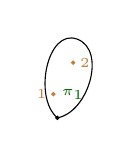
\begin{tikzpicture}
\draw [name path=pi1] (0,0) to [out=10,in=-20] (0.25,1) to [out=160,in=140] cycle node(o) {}; 
\draw (o) circle[fill, radius=0.02];
\node [black!60!green] at (0.2,0.3) {\tiny{$\pi_1$}};
\draw [fill, brown] (-.05,0.3) circle [radius=0.02];
\node [brown] at (-.2,0.3) {\tiny{1}};
\draw [fill, brown] (0.2,0.7) circle [radius=0.02];
\node [brown] at (.35,.7) {\tiny{2}};
\end{tikzpicture},
\quad $\hat{f}_T($
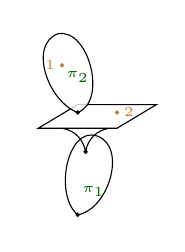
\begin{tikzpicture}
\draw (0,0) to [out=10,in=-20] (0.25,1) to [out=160,in=140] cycle node(o) {}; 
\draw (o) circle[fill, radius=0.02];
\draw (-0.2,1.1) to [out=-10,in=100] ++(0.3,-0.3) node(o2){} to [out=80,in=190] ++(0.3,0.3);
\draw (o2) circle[fill, radius=0.02];
\filldraw [fill=white, fill opacity=0.8] ($(o2)+(-0.6,0.3)$) -- ++(1,0) -- ++(0.5,0.3) -- ++(-1,0) --cycle;
\filldraw [fill=white, fill opacity=0.8] (0,1.3) coordinate(o3) to [out=20,in=10] ++(-.25,1) to [out=200,in=160] cycle; 
\draw (o3) circle[fill, radius=0.02];
\node [black!60!green] at (0.2,0.3) {\tiny{$\pi_1$}};
\node [black!60!green] at ($(o3)+(0,0.45)$) {\tiny{$\pi_2$}};
\draw [fill, brown] ($(o3)+(-0.2,0.6)$) node(p1){} circle [radius=0.02];
\node [brown] at ($(p1)+(-0.15,0)$) {\tiny{1}};
\draw [fill, brown] ($(o2)+(.4,0.5)$) node(p2){} circle [radius=0.02];
\node [brown] at ($(p2)+(0.15,0)$) {\tiny{2}};
\end{tikzpicture}
$)=$
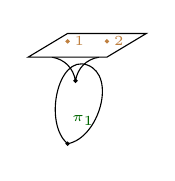
\begin{tikzpicture}
\draw (0,0) to [out=10,in=-20] (0.25,1) to [out=160,in=140] cycle node(o) {}; 
\draw (o) circle[fill, radius=0.02];
\draw (-0.2,1.1) to [out=-10,in=100] ++(0.3,-0.3) node(o2){} to [out=80,in=190] ++(0.3,0.3);
\draw (o2) circle[fill, radius=0.02];
\filldraw [fill=white, fill opacity=0.8] ($(o2)+(-0.6,0.3)$) -- ++(1,0) -- ++(0.5,0.3) -- ++(-1,0) --cycle;
\node [black!60!green] at (0.2,0.3) {\tiny{$\pi_1$}};
\draw [fill,brown] (0,1.3) node(p1){} circle [radius=0.02];
\node [brown] at ($(p1)+(0.15,0)$) {\tiny{1}};
\draw [fill, brown] ($(o2)+(.4,0.5)$) node(p2){} circle [radius=0.02];
\node [brown] at ($(p2)+(0.15,0)$) {\tiny{2}};
\end{tikzpicture},
\quad $\hat f_{T'}($
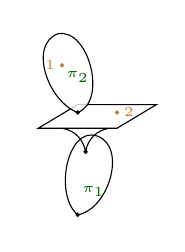
\begin{tikzpicture}
\draw (0,0) to [out=10,in=-20] (0.25,1) to [out=160,in=140] cycle node(o) {}; 
\draw (o) circle[fill, radius=0.02];
\draw (-0.2,1.1) to [out=-10,in=100] ++(0.3,-0.3) node(o2){} to [out=80,in=190] ++(0.3,0.3);
\draw (o2) circle[fill, radius=0.02];
\filldraw [fill=white, fill opacity=0.8] ($(o2)+(-0.6,0.3)$) -- ++(1,0) -- ++(0.5,0.3) -- ++(-1,0) --cycle;
\filldraw [fill=white, fill opacity=0.8] (0,1.3) coordinate(o3) to [out=20,in=10] ++(-.25,1) to [out=200,in=160] cycle; 
\draw (o3) circle[fill, radius=0.02];
\node [black!60!green] at (0.2,0.3) {\tiny{$\pi_1$}};
\node [black!60!green] at ($(o3)+(0,0.45)$) {\tiny{$\pi_2$}};
\draw [fill, brown] ($(o3)+(-0.2,0.6)$) node(p1){} circle [radius=0.02];
\node [brown] at ($(p1)+(-0.15,0)$) {\tiny{1}};
\draw [fill, brown] ($(o2)+(.4,0.5)$) node(p2){} circle [radius=0.02];
\node [brown] at ($(p2)+(0.15,0)$) {\tiny{2}};
\end{tikzpicture}
$)=$
\begin{tikzpicture}
%\node(o2) at (0.1,0.8) {}; 
\filldraw [fill=white, fill opacity=0.8] ($(0.1,0.8)+(-0.6,0.3)$) -- ++(1,0) -- ++(0.5,0.3) -- ++(-1,0) --cycle;
\draw [fill,brown] (0,1.3) node(p1){} circle [radius=0.02];
\node [brown] at ($(p1)+(-0.15,0)$) {\tiny{1}};
\draw [fill, brown] ($(o2)+(.4,0.5)$) node(p2){} circle [radius=0.02];
\node [brown] at ($(p2)+(0.15,0)$) {\tiny{2}};
\end{tikzpicture}. 
\end{eg}

\begin{eg}[$|B|=2$, in $\wt{C}_2$]
$T=\begin{tikzpicture}
\node [below] at (0,0) {\tiny{r}};  
\node [right, black!60!green] at (0,0) {\tiny{$\pi_1$}};
\node [left, brown] at (0,0) {\tiny{1,2}};
\node [right, black!60!green] at (0,0.5) {\tiny{$\pi_2$}};
\draw [fill] (0,0) circle [radius=0.02];
\draw [fill] (0,0.5) circle [radius=0.02];
\draw (0,0) -- (0,0.5);
\end{tikzpicture}$, 
$T'=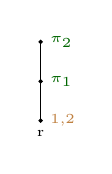
\begin{tikzpicture}
\node [below] at (0,0) {\tiny{r}};  
\node [right,brown] at (0,0) {\tiny{1,2}};
\node [right, black!60!green] at (0,0.5) {\tiny{$\pi_1$}};
\node [right, black!60!green] at (0,1) {\tiny{$\pi_2$}};
\draw [fill] (0,0) circle [radius=0.02];
\draw [fill] (0,0.5) circle [radius=0.02];
\draw [fill] (0,1) circle [radius=0.02];
\draw (0,0) -- (0,0.5) -- (0,1);
\end{tikzpicture}$ 
(so $\cS_{T'}\subset\ov{\cS}_T$), 

$\hat{f}_T($
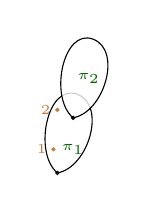
\begin{tikzpicture}
\draw (0,0) to [out=10,in=-20] (0.25,1) to [out=160,in=140] cycle node(o) {}; 
\draw (o) circle[fill, radius=0.02];
\filldraw [fill=white, fill opacity=0.8] (0.2,0.7) coordinate(o2) to [out=10,in=-20] ++(0.25,1) to [out=160,in=140] cycle; 
\draw (o2) circle[fill, radius=0.02];
\node [black!60!green] at (0.2,0.3) {\tiny{$\pi_1$}};
\node [black!60!green] at (0.4,1.2) {\tiny{$\pi_2$}};
\draw [fill, brown] (-.05,0.3) circle [radius=0.02];
\node [brown] at (-.2,0.3) {\tiny{1}};
\draw [fill, brown] (0,0.8) circle [radius=0.02];
\node [brown] at (-.15,0.8) {\tiny{2}};
\end{tikzpicture}
$)=$
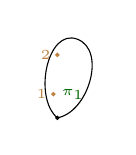
\begin{tikzpicture}
\draw [name path=pi1] (0,0) to [out=10,in=-20] (0.25,1) to [out=160,in=140] cycle node(o) {}; 
\draw (o) circle[fill, radius=0.02];
\node [black!60!green] at (0.2,0.3) {\tiny{$\pi_1$}};
\draw [fill, brown] (-.05,0.3) circle [radius=0.02];
\node [brown] at (-.2,0.3) {\tiny{1}};
\draw [fill, brown] (0,0.8) circle [radius=0.02];
\node [brown] at (-.15,0.8) {\tiny{2}};
\end{tikzpicture},
\quad $\hat{f}_T($
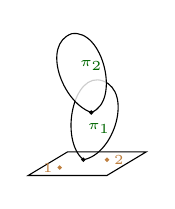
\begin{tikzpicture}
\coordinate (o2) at (0,0); 
\filldraw [fill=white, fill opacity=0.8] ($(o2)$) -- ++(1,0) -- ++(0.5,0.3) -- ++(-1,0) --cycle;

\draw (0.7,0.2) to [out=10,in=-20] ++(0.25,1) to [out=160,in=140] cycle node(o) {}; 
\draw (o) circle[fill, radius=0.02];

\filldraw [fill=white, fill opacity=0.8] (0.8,0.8) coordinate(o3) to [out=20,in=10] ++(-.25,1) to [out=200,in=160] cycle; 
\draw (o3) circle[fill, radius=0.02];


\node [black!60!green] at ($(o)+(0.2,0.4)$) {\tiny{$\pi_1$}};
\node [black!60!green] at ($(o3)+(0,0.6)$) {\tiny{$\pi_2$}};
\draw [fill, brown] ($(o2)+(0.4,0.1)$) node(p1){} circle [radius=0.02];
\node [brown] at ($(p1)+(-0.15,0)$) {\tiny{1}};
\draw [fill, brown] ($(o2)+(1,0.2)$) node(p2){} circle [radius=0.02];
\node [brown] at ($(p2)+(0.15,0)$) {\tiny{2}};
\end{tikzpicture}
$)=$
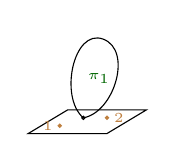
\begin{tikzpicture}
\coordinate (o2) at (0,0); 
\filldraw [fill=white, fill opacity=0.8] ($(o2)$) -- ++(1,0) -- ++(0.5,0.3) -- ++(-1,0) --cycle;

\draw (0.7,0.2) to [out=10,in=-20] ++(0.25,1) to [out=160,in=140] cycle node(o) {}; 
\draw (o) circle[fill, radius=0.02];

\node [black!60!green] at ($(o)+(0.2,0.5)$) {\tiny{$\pi_1$}};
\draw [fill, brown] ($(o2)+(0.4,0.1)$) node(p1){} circle [radius=0.02];
\node [brown] at ($(p1)+(-0.15,0)$) {\tiny{1}};
\draw [fill, brown] ($(o2)+(1,0.2)$) node(p2){} circle [radius=0.02];
\node [brown] at ($(p2)+(0.15,0)$) {\tiny{2}};
\end{tikzpicture}
\quad $\hat f_{T'}($
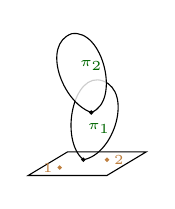
\begin{tikzpicture}
\coordinate (o2) at (0,0); 
\filldraw [fill=white, fill opacity=0.8] ($(o2)$) -- ++(1,0) -- ++(0.5,0.3) -- ++(-1,0) --cycle;

\draw (0.7,0.2) to [out=10,in=-20] ++(0.25,1) to [out=160,in=140] cycle node(o) {}; 
\draw (o) circle[fill, radius=0.02];

\filldraw [fill=white, fill opacity=0.8] (0.8,0.8) coordinate(o3) to [out=20,in=10] ++(-.25,1) to [out=200,in=160] cycle; 
\draw (o3) circle[fill, radius=0.02];


\node [black!60!green] at ($(o)+(0.2,0.4)$) {\tiny{$\pi_1$}};
\node [black!60!green] at ($(o3)+(0,0.6)$) {\tiny{$\pi_2$}};
\draw [fill, brown] ($(o2)+(0.4,0.1)$) node(p1){} circle [radius=0.02];
\node [brown] at ($(p1)+(-0.15,0)$) {\tiny{1}};
\draw [fill, brown] ($(o2)+(1,0.2)$) node(p2){} circle [radius=0.02];
\node [brown] at ($(p2)+(0.15,0)$) {\tiny{2}};
\end{tikzpicture}
$)=$
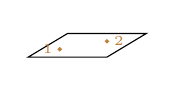
\begin{tikzpicture}
\coordinate (o2) at (0,0); 
\filldraw [fill=white, fill opacity=0.8] ($(o2)$) -- ++(1,0) -- ++(0.5,0.3) -- ++(-1,0) --cycle;
\draw [fill, brown] ($(o2)+(0.4,0.1)$) node(p1){} circle [radius=0.02];
\node [brown] at ($(p1)+(-0.15,0)$) {\tiny{1}};
\draw [fill, brown] ($(o2)+(1,0.2)$) node(p2){} circle [radius=0.02];
\node [brown] at ($(p2)+(0.15,0)$) {\tiny{2}};
\end{tikzpicture}. 

\end{eg}

\begin{eg}[$|B|=1$, in $\ov{C}_2(\pi)$ where $\pi$ is an $(M,\infty)$-bundle]\label{fhatB1_eg}
$T_1=$
\begin{tikzpicture}
\node [below] at (0,0) {\tiny{r}};  
\node [right, black!60!green] at (0,0) {\tiny{$\pi$}};
\node [right, brown] at (0,0.5) {\tiny{1,2}};
\draw [fill] (0,0) circle [radius=0.02];
\draw [fill] (0,0.5) circle [radius=0.02];
\draw (0,0) -- (0,0.5);
\end{tikzpicture}, 
$T_2=$
\begin{tikzpicture}
\node [below] at (0,0) {\tiny{r}};  
\node [right, brown] at (0,0) {\tiny{1,2}};
\node [right, black!60!green] at (0,0.5) {\tiny{$\pi$}};
\draw [fill] (0,0) circle [radius=0.02];
\draw [fill] (0,0.5) circle [radius=0.02];
\draw (0,0) -- (0,0.5);
\end{tikzpicture}, 
$T_3=$
\begin{tikzpicture}
\node [below] at (0,0) {\tiny{r}};  
\node [left, brown] at (0,0) {\tiny{2}};
\node [right, black!60!green] at (0,0.5) {\tiny{$\pi$}};
\node [left, brown] at (0,0.5) {\tiny{1}};
\draw [fill] (0,0) circle [radius=0.02];
\draw [fill] (0,0.5) circle [radius=0.02];
\draw (0,0) -- (0,0.5);
\end{tikzpicture},

$\hat{f}_{T_1}($
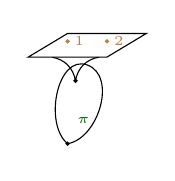
\begin{tikzpicture}
\draw (0,0) to [out=10,in=-20] (0.25,1) to [out=160,in=140] cycle node(o) {}; 
\draw (o) circle[fill, radius=0.02];
\draw (-0.2,1.1) to [out=-10,in=100] ++(0.3,-0.3) node(o2){} to [out=80,in=190] ++(0.3,0.3);
\draw (o2) circle[fill, radius=0.02];
\filldraw [fill=white, fill opacity=0.8] ($(o2)+(-0.6,0.3)$) -- ++(1,0) -- ++(0.5,0.3) -- ++(-1,0) --cycle;
\node [black!60!green] at (0.2,0.3) {\tiny{$\pi$}};
\draw [fill,brown] (0,1.3) node(p1){} circle [radius=0.02];
\node [brown] at ($(p1)+(0.15,0)$) {\tiny{1}};
\draw [fill, brown] ($(o2)+(.4,0.5)$) node(p2){} circle [radius=0.02];
\node [brown] at ($(p2)+(0.15,0)$) {\tiny{2}};
\end{tikzpicture}
$)=$
\begin{tikzpicture}
%\node(o2) at (0.1,0.8) {}; 
\filldraw [fill=white, fill opacity=0.8] ($(0.1,0.8)+(-0.6,0.3)$) -- ++(1,0) -- ++(0.5,0.3) -- ++(-1,0) --cycle;
\draw [fill,brown] (0,1.3) node(p1){} circle [radius=0.02];
\node [brown] at ($(p1)+(0.15,0)$) {\tiny{1}};
\draw [fill, brown] ($(o2)+(.4,0.5)$) node(p2){} circle [radius=0.02];
\node [brown] at ($(p2)+(0.15,0)$) {\tiny{2}};
\end{tikzpicture}, 
\quad$\hat{f}_{T_2}($
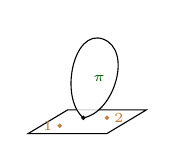
\begin{tikzpicture}
\filldraw [fill=white, fill opacity=0.8] ($(-0.7,-0.2)$) -- ++(1,0) -- ++(0.5,0.3) -- ++(-1,0) --cycle;
\filldraw [fill=white, fill opacity=0.8] (0,0) coordinate(o2) to [out=10,in=-20] ++(0.25,1) to [out=160,in=140] cycle; 
\draw (o2) circle[fill, radius=0.02];
\node [black!60!green] at ($(o2)+(0.2,0.5)$) {\tiny{$\pi$}};
\draw [fill,brown] (-0.3,-0.1) node(p1){} circle [radius=0.02];
\node [brown] at ($(p1)+(-0.15,0)$) {\tiny{1}};
\draw [fill, brown] (0.3,0) node(p2){} circle [radius=0.02];
\node [brown] at ($(p2)+(0.15,0)$) {\tiny{2}};
\end{tikzpicture}
$)=$
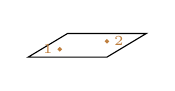
\begin{tikzpicture}
\filldraw [fill=white, fill opacity=0.8] ($(-0.7,-0.2)$) -- ++(1,0) -- ++(0.5,0.3) -- ++(-1,0) --cycle;
\draw [fill,brown] (-0.3,-0.1) node(p1){} circle [radius=0.02];
\node [brown] at ($(p1)+(-0.15,0)$) {\tiny{1}};
\draw [fill, brown] (0.3,0) node(p2){} circle [radius=0.02];
\node [brown] at ($(p2)+(0.15,0)$) {\tiny{2}};
\end{tikzpicture}, 
\quad$\hat{f}_{T_3}($
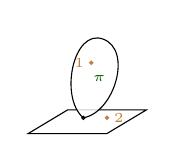
\begin{tikzpicture}
\filldraw [fill=white, fill opacity=0.8] ($(-0.7,-0.2)$) -- ++(1,0) -- ++(0.5,0.3) -- ++(-1,0) --cycle;
\filldraw [fill=white, fill opacity=0.8] (0,0) coordinate(o2) to [out=10,in=-20] ++(0.25,1) to [out=160,in=140] cycle; 
\draw (o2) circle[fill, radius=0.02];
\node [black!60!green] at ($(o2)+(0.2,0.5)$) {\tiny{$\pi$}};
\draw [fill,brown] (0.1,0.7) node(p1){} circle [radius=0.02];
\node [brown] at ($(p1)+(-0.15,0)$) {\tiny{1}};
\draw [fill, brown] (0.3,0) node(p2){} circle [radius=0.02];
\node [brown] at ($(p2)+(0.15,0)$) {\tiny{2}};
\end{tikzpicture}
$)=$
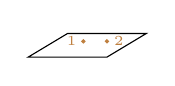
\begin{tikzpicture}
\filldraw [fill=white, fill opacity=0.8] ($(-0.7,-0.2)$) -- ++(1,0) -- ++(0.5,0.3) -- ++(-1,0) --cycle;
\draw [fill,brown] (0,0) node(p1){} circle [radius=0.02];
\node [brown] at ($(p1)+(-0.15,0)$) {\tiny{1}};
\draw [fill, brown] (0.3,0) node(p2){} circle [radius=0.02];
\node [brown] at ($(p2)+(0.15,0)$) {\tiny{2}};
\end{tikzpicture}. 

Note that $S_{T_1},S_{T_2},S_{T_3}$ are the only codimension-1 strata of $\ov{C}_2(\pi)$, and the codomain of $\hat{f}_{T_1}$, $\hat{f}_{T_2}$, $\hat{f}_{T_3}$ are all $\ov{C}_2(\R^d)$. 
\end{eg}

\begin{crl}[of Lemma \ref{treecontr1_lmm}]\label{treecontr2_crl}
Let $T',T$ be $(\{1,2\},B)$-labeled trees such that $T$ can be obtained from $T'$ by contracting some edges, then $\fc_{T',T}(\nu_{T'})=\nu_T$. 
Moreover, if $\fs_T=\R^d$, then $\fs_{T'}=\R^d$. 
\end{crl}

The following lemma is easy to check: \footnote{Hint: By continuity of the $\hat{f}$ maps, it suffices to prove the equality on the open part $\cS_{T'}$.}
\begin{lmm}\label{treecontr3_lmm}
Let $T',T$ be $(\{1,2\},B)$-labeled trees such that $T$ can be obtained from $T'$ by contracting some edges, then
$$\hat{f}_{T'}=\hat{f}_{G_{T',T}}\circ(\hat{f}_{T}|_{\ov\cS_{T'}}).$$
\end{lmm}

\begin{dfn}\label{propagator_dfn}
Suppose $M$ is a $d$-dimensional $\Z$-homology sphere and $\pi$ is an $(M,\infty)$-bundle. 
A {\it propagator} on $\ov{C}_2(\pi)$ (resp. $\ov{C}_2(\R^d)$) is a closed $(d-1)$-form $\omega$ on $\ov{C}_2(\pi)$ satisfying: there exists a $(d-1)$-form $\omega_0$ on $S^{d-1}\approx\ov{C}_2(\R^d)$ such that $\int_{S^{d-1}}\omega_0=1$ and for every codimension-1 stratum $S\subset\partial\ov{C}_2(\pi)$ (resp. $S\subset\partial\ov{C}_2(\R)$), $\omega|_{\ov{S}}=\hat{f}_{\cT_S}^*\omega_0$. 
\end{dfn}

This definition is phrased differently from the usual definition of a propagator, see e.g. \cite[Definition 3.9]{Lescop} or \cite[Lemma 2.12]{WatanabeAddendum}, but can easily be seen to be equivalent. 

Fix a volume form $\omega_0$ on $S^{d-1}$. 
By \cite[Lemma 2.12]{WatanabeAddendum}, there exist propagators $\omega_1$ on $\ov{C}_2(\pi_1)$, $\omega_2$ on $\ov{C}_2(\pi_2)$, and $\omega$ on $\ov{C}_2([\pi_1,\pi_2])$ such that the above condition in Definition \ref{propagator_dfn} is satisfied with this $\omega_0$. We choose and fix such $\omega_1,\omega_2,\omega$. 

In the rest of this section we construct a ``propagator'' on $\partial\wt{C}_2$. 
This is done in two steps: 
\begin{enumerate}
\item \label{step1_item} On each stratum $S$ of $\partial\wt{C}_2$, construct a closed $(d-1)$-form $\omega_S$ on $\ov{S}$, such that, for two strata $S'\subset\ov{S}$, $\omega_S|_{\ov{S}'}=\omega_{S'}$. 
\item \label{step2_item} Show that this collection $\{\omega_S\}_S$ extends to a closed form $\wt\omega$ on $\wt{C}_2$; namely, $\wt\omega$ is such that $\wt\omega|_{S}=\omega_S$ for every strata $S\subset\partial\wt{C}_2$. 
\end{enumerate}

{\bf Step \ref{step1_item}}: 
There are two kinds of strata in $\partial\wt{C}_2$: those that are not subsets of $\ov{S}_{\sgray}$ and those that are. 
The former kind of strata are of the form $\cS_T$ for some unique $(\{1,2\},\{\pi_1,\pi_2\})$-labeled tree $T$ with at least one edge. 
For these strata, define $\omega_{\cS_T}=\hat{f}_T^*\omega_i$, where $i=1$ if $\fs_T=\pi_1$, $i=2$ if $\fs_T=\pi_2$, $i=0$ if $\fs_T=\R^d$, and remove the subscript $i$ if $\fs_T=[\pi_1,\pi_2]$. 
For the latter kind of strata: under the natural identification $\ov{S}_\sgray\approx\ov{C}_2([\pi_1,\pi_2])$, define $\omega_S$ to be the restriction of $\omega$ to $S$. 
This defines the collection $\{\omega_S\}_{S}$.

Now we need to show the compatibility condition:
for $S'\subset\ov{S}$, $\omega_S|_{\ov{S}'}=\omega_{S'}$. 
%Since $\omega_{S}, \omega_{S'}$ are continuous, it suffices to show equality on the open part:  $\omega_S|_{S'}=\omega_{S'}|_{S'}$. 

\begin{itemize}
\item If $S',S\subset\ov{S}_{\sgray}$, then this holds by definition. 

\item 
If $S',S\not\subset\ov{S}_{\sgray}$: since $\omega_S=\hat{f}_{\cT_S}\omega_i$ for some propagator $\omega_i$, 
%and $\omega_{S'}=\hat{f}_{\cT_{S'}}\omega_{i'}$,
$$\omega_S|_{\ov{S}'}=(\hat{f}_{\cT_S}|_{\ov{S}'})^*\omega_i=
\begin{cases}
\hat{f}_{\cT_{S'}}^*\omega_{i}, 
\tn{ if } G_{\cT_{S'},\cT_S} \tn{ has only 1 vertex}
\\
(\hat{f}_{\cT_S}|_{\ov{S}'})^*\hat{f}_{G_{\cT_{S'},\cT_S}}^*\omega_0=\hat{f}_{\cT_{S'}}^*\omega_{0}, \tn{ otherwise}
\end{cases}
=\omega_{S'},$$
where, for the second case, the second equality is because $\omega_i$ is a propagator as in Definition \ref{propagator_dfn} and the third equality is because of Lemma \ref{treecontr4_lmm}. 

\item If $S'\subset\ov{S}_{\sgray}$, $S\not\subset\ov{S}_{\sgray}$: 
let $T'$ be the $(\{1,2\},\{[\pi_1,\pi_2]\})$-labeled tree $\cT_{S'}$ under the identification $\ov{S}_{\sgray}\approx\ov{C}_2([\pi_1,\pi_2])$. 
We can also view $T'$ as a $(\{1,2\},\{\pi_1,\pi_2\})$-labeled tree; to avoid confusion let us call this $(\{1,2\},\{\pi_1,\pi_2\})$-tree $T$. 
Then $\cS_{T}\subset\ov{S}_{\sblue}$ is a stratum of $\wt{C}_2$, 
$\cS_{T}\subset S$ and $\cS_{T}\cap\ov{S}_{\sgray}=S'$. 
Since we have already shown $\omega_S|_{\ov{\cS}_{T}}=\omega_{\cS_{T}}$, it suffices to show $\omega_{\cS_{T}}|_{\ov{S}'}=\omega_{S'}$. 
We first state a lemma: 
\begin{lmm}\label{treecontr4_lmm}
Let $S$ be a stratum of $\partial\wt{C}_2$. 
If $S\subset\ov{S}_{\sblue}$ and $S\not\subset\ov{S}_{\sgray}$, then $\fs_{\cT_S}=\R^d$. 
\end{lmm}
\begin{proof}
If $S$ is of top dimension in $\ov{S}_{\sblue}$, then $\cT_S$ has one vertex with space label $[\pi_1,\pi_2]$ and only one edge. 
The statement of the lemma follows from the last sentence of Example \ref{fhatB1_eg}. 
If $S$ is not of top dimension in $\ov{S}_{\sblue}$, then it is in the closure of a stratum of top dimension, and the lemma follows from the last sentence of Corollary \ref{treecontr2_crl}. 
\end{proof}
Now, because the definition of $\hat{f}$ is combinatorial and $T,T'$ are the same tree, the two maps 
$$\hat{f}_{T}|_{\ov{S}'}:\ov{S}'\longrightarrow\ov{C}_2(\R^d),\qquad
\hat{f}_{T'}:\ov{S}'\longrightarrow\ov{C}_2(\R^d)$$
are equal, 
where the first $\ov{S}'$ is viewed as a subset of the stratum $\ov{\cS}_T$ in $\wt{C}_2$ while the second $\ov{S}'$ is viewed as a boundary stratum of $\ov{C}_2([\pi_1,\pi_2])$ under the identification 
$\ov{S}_{\sgray}\approx\ov{C}_2([\pi_1,\pi_2])$.
%The codomain of the first map is $\ov{C}_2(\R^d)$ because of Lemma \ref{treecontr4_lmm} and the codomain of the second map is $\ov{C}_2(\R^d)$ because $\ov{S}'\neq\ov{S}_{\sgray}$.
Since $\omega_{\cS_{T}}=\hat{f}_{T}^*\omega_0$ and $\omega_{S'}=\hat{f}_{T'}\omega_0$, we conclude that they are equal on $\ov{S}'$. 
\end{itemize}


~\\
{\bf Step 2:} The following statement (Corollary \ref{formextension_crl}) is proved in Appendix \ref{fromextension_appendix}: 

{\it Suppose $M$ is a compact manifold with embedded faces such that $H^k(M;\R)\to H^k(\partial M;R)$ is surjective. Suppose for every stratum $S\subset\partial{M}$, $\omega_S$ is a closed $k$-form on $S$, such that, if $S'\subset \ov{S}$, then $\omega_S|_{S'}=\omega_{S'}$. 
Then, there exists a closed $k$-form $\wt{\omega}$ on $M$ such that $\wt{\omega}|_{S}=\omega_S$ for every $S$.}

Therefore, to show the existence of a closed form $\wt{\omega}$ on $\wt{C}_2$ extending the $\{\omega_S\}_S$ we just defined, 
it suffices to show that the map 
$$H^{d-1}(\wt{C}_2)\xrightarrow{\tn{restriction}}H^{d-1}(\partial\wt{C}_2)$$
is surjective. 
It is therefore sufficient to show that $H^d(\wt{C}_2,\partial\wt{C}_2)=0$. But 
\begin{align*}
H^*(\wt{C}_2,\partial\wt{C}_2)\approx
H_{\dim(\wt{C}_2)-*}(\wt{C}_2-\partial\wt{C}_2)=
H_{\dim(\wt{C}_2)-*}\big(C_2([\pi_1,\pi_2])\times (0,1)\big)\\
\approx
H_{\dim(\wt{C}_2)-*}({C}_2([\pi_1,\pi_2]))
\approx H^{*-1}\big(\ov{C}_2([\pi_1,\pi_2]),\partial\ov{C}_2([\pi_1,\pi_2])\big), 
\end{align*}
%$\dim(\wt{C}_2)=\dim(C_2([\pi_1,\pi_2]))+1=3d+1+\dim(B_1)+\dim(B_2)$ 
and this is 0 when $*-1<d+1$ by the proof of Lemma 2.12 in \cite{WatanabeAddendum}. 

We choose and fix such an extension $\wt\omega$ on $\wt{C}_2$. 

\section{Configuration space integrals}

Note that $B_I$ as defined in conftilde Section 2.4 admits a submersion $\pi_{B_I}:B_I\to B_1\times B_2$, making $B_I$ a smooth fiber bundle (whose fibers are manifolds with corners) over $B_1\times B_2$. Each fiber is homeomorphic to $S^d\times [0,\rho)$ and looks like the picture on page 10 of conftilde. 
The map $\pi_{B_I}\circ\tilde{\pi}^A:\wt{C}_A\to B_1\times B_2$, and its restriction to every strata of $\wt{C}_A$, are also submersions. 

The base $B$ of $[\pi_1,\pi_2]$ is $B_{t_0}$, 
the total space of the subbundle of $B_I$ obtained by taking the subspace $S^d\times \{t_0\}\subset S^d\times[0,\rho)$ of each fiber. So, the fibers are diffeomorphic to $S^d$. 
Indeed, the fiber bundle $B\to B_1\times B_2$ is trivial when regarded as a topological fiber bundle; namely, $B$ is homeomorphic to $S^d\times B_1\times B_2$. So, 
%With the Leray-Serre spectral sequence we compute 
$H^*(B)\approx H^*(S^d)\otimes H^*(B_1)\otimes H^*(B_2)$. 



We have the following diagram: 
\[
\begin{tikzcd}
\ov{C}_A([\pi_1,\pi_2])\rar[hook]\dar["\pi_{[]}^A"] & \wt{C}_A\dar["\tilde\pi^A"]\\
B_{t_0}\rar[hook]\drar["\pi_{B_I}|_{B_{t_0}}"'] & B_I\dar["\pi_{B_I}"] \\
 & B_1\times B_2
\end{tikzcd},
\]
where $\pi_{[]}^A$, $\pi_{B_I}$ are submersions but not $\tilde\pi^A$. 

\begin{lmm}
Let $A'\subset A$ be finite sets and $\ff_{A',A}:\wt{C}_{A}\to\wt{C}_{A'}$ the forgetful map forgetting all marked points not in $A'$. 
Then, for every (open) stratum $S$ of $\wt{C}_{A}$, $\ff_{A',A}(S)$ is again an open stratum of $\wt{C}_{A'}$ and 
$$\ff_{A',A}|_S:S\longrightarrow \ff_{A',A}(S)$$
is a submersion. 
\end{lmm}

In particular, when $A'=\emptyset$, this holds with $\wt{C}_{A'}=B_I$ and $\ff_{A',A}=\tilde{\pi}$. 

\cmt{Something about the above should be in the conftilde section.}


Suppose $\sum_{i=1}^{m}\Gamma_i$ is a cocycle in graph cohomology. 
For every edge $e$ of some $\Gamma_i$, we have the forgetful map 
$$\ff_e:\wt{C}_{V(\Gamma_i)}\longrightarrow\wt{C}_2.$$
And, when restricted to $\ov{S}_{\sgray}\subset\wt{C}_{V(\Gamma_i)}$ (resp. $\ov{C}_{V(\Gamma_i)}^*\subset\wt{C}_{V(\Gamma_i)}$), it is the forgetful map
$$\ff_e:\ov{C}_{V(\Gamma_i)}([\pi_1,\pi_2])\longrightarrow\ov{C}_2([\pi_1,\pi_2]) \qquad (\tn{resp. } \ff_e:\ov{C}^*_{V(\Gamma_i)}\longrightarrow\ov{C}^*_2).$$
Now we have the form $\bigwedge_{e\in E(\Gamma_i)}\ff_e^*\wt{\omega}$ on $\wt{C}_{V(\Gamma_i)}$. 
Recall that by the definition of Kontsevich's characteristic classes, 
$$K_{[\pi_1,\pi_2]}\big(\big[\sum_{i=1}^m\Gamma_i\big]\big)=
\big[\sum_{i=1}^m (\pi_{[]}^{V(\Gamma_i)})_*\bigwedge_{e\in E(\Gamma_i)}\ff_e^*{\omega}\big]\in H^*(B)\approx H^*(S^d)\otimes H^*(B_1)\otimes H^*(B_2).
%\sum_{i=1}^m\int_{\ov{S}_{\sgray}}\bigwedge_{e\in E(\Gamma_i)}\ff_e^*\wt{\omega}|_{\ov{S}_{\sgray}}.
$$
To determine $K_{[\pi_1,\pi_2]}\big(\big[\sum_{i=1}^m\Gamma_i\big]\big)$, it suffices to determine the intersection pairing 
$$\big\langle K_{[\pi_1,\pi_2]}\big(\big[\sum_{i=1}^m\Gamma_i\big]\big), \alpha_0\otimes\alpha_1\otimes\alpha_2\big\rangle$$
for all homology classes $\alpha_0\in H_*(S^d)$, $\alpha_1\in H_*(B_1)$ and $\alpha_2\in H_*(B_2)$. 
Below, we discuss the two cases $\alpha_0=[\tn{point}]$ and $\alpha_0=[S^d]$ separately. 

\subsection*{Case I: $\alpha_0=[S^d]$}

For $a=1,2$, suppose $\deg\alpha_a=k_a$ and $\alpha_a$ is represented by a piecewise-smooth singular chain $\sum_{j_a}\iota^{j_a}_a$, 
where $\iota^{j_a}_a$ are smooth maps from the standard $k_a$-dimensional simplex $\Delta^{k_a}$ to $B_a$. 

Since for all finite set $A$,
$\pi_{B_I}\circ\tilde{\pi}^A:\wt{C}_A\to B_1\times B_2$
and its restriction to every stratum is a fiber bundle, 
we can form the pullback bundles $(\iota_1^{j_1},\iota_2^{j_2})^*\wt{C}_A$, $(\iota_1^{j_1},\iota_2^{j_2})^*\ov{C}_A([\pi_1,\pi_2])$ ,$(\iota_1^{j_1},\iota_2^{j_2})^*\ov{C}^*_A$ over $\Delta^{k_1}\times\Delta^{k_2}$. 

For convenience, in this section we use $\ov{S}_{\sgray}^i$ to denote the $\ov{S}_{\sgray}$ in $\wt{C}_{V(\Gamma_i)}$, and same for the other colors (red, orange, yellow, blue) instead of gray. 

We then have 
\begin{equation}
\label{integral_eqn}
\big\langle K_{[\pi_1,\pi_2]}([\sum_{i=1}^m\Gamma_i]), [S^d]\otimes\alpha_1\otimes\alpha_2 \big\rangle=
\sum_{i,j_1,j_2}\int_{(\iota_1^{j_1},\iota_2^{j_2})^*\ov{C}_{V(\Gamma_i)}([\pi_1,\pi_2])}\bigwedge_{e}\ff_e^*{\omega}=
\sum_{i,j_1,j_2}\int_{(\iota_1^{j_1},\iota_2^{j_2})^*\ov{S}_{\sgray}^i}\bigwedge_{e}\ff_e^*\wt{\omega}.
\end{equation}
Since 
\[
\partial\big((\iota_1^{j_1},\iota_2^{j_2})^*\wt{C}_{V(\Gamma_i)}\big)=(\iota_1^{j_1},\iota_2^{j_2})^*\partial\wt{C}_{V(\Gamma_i)}+\big((\iota_1^{j_1},\iota_2^{j_2})^*\wt{C}_{V(\Gamma_i)}\big)\big|_{\partial(\Delta^{k_1}\times\Delta^{k_2})}, 
\]
by Stocks' Formula, 
\begin{align*}
\int_{(\iota_1^{j_1},\iota_2^{j_2})^*\partial\wt{C}_{V(\Gamma_i)}}\bigwedge_{e}&\ff_e^*\wt{\omega}=
\int_{\partial(\iota_1^{j_1},\iota_2^{j_2})^*\wt{C}_{V(\Gamma_i)}}\bigwedge_{e}\ff_e^*\wt{\omega}-
\int_{(\iota_1^{j_1},\iota_2^{j_2})^*\wt{C}_{V(\Gamma_i)}|_{\partial(\Delta^{k_1}\times\Delta^{k_2})}}\bigwedge_{e}\ff_e^*\wt{\omega}\\
=\int_{(\iota_1^{j_1},\iota_2^{j_2})^*\wt{C}_{V(\Gamma_i)}}&d\Big(\bigwedge_{e}\ff_e^*\wt{\omega}\Big)-
\int_{(\iota_1^{j_1},\iota_2^{j_2})^*\wt{C}_{V(\Gamma_i)}|_{\partial\Delta^{k_1}\times\Delta^{k_2}}}\bigwedge_{e}\ff_e^*\wt{\omega}\pm
\int_{(\iota_1^{j_1},\iota_2^{j_2})^*\wt{C}_{V(\Gamma_i)}|_{\Delta^{k_1}\times\partial\Delta^{k_2}}}\bigwedge_{e}\ff_e^*\wt{\omega}.
\end{align*}
The first term is 0 because $\wt{\omega}$ is closed.  
Because the singular chains $\sum_{j_1}\iota_1^{j_1}$, $\sum_{j_2}\iota_2^{j_2}$ are cycles, when summing over all $j_1$, the second term is 0; when summing over all $j_2$, the third term is 0. 
So, 
$$(\ref{integral_eqn})=\sum_{i,j_1,j_2}\Big(\int_{(\iota_1^{j_1},\iota_2^{j_2})^*\ov{S}_{\sblue}^i}\bigwedge_{e}\ff_e^*\wt{\omega}+\int_{(\iota_1^{j_1},\iota_2^{j_2})^*\ov{C}^*_{V(\Gamma_i)}}\bigwedge_{e}\ff_e^*{\wt\omega}\Big).$$
Since $\sum_{i}\Gamma_i$ is a cocycle in graph cohomology, the first term is 0 just like in the proof of the well-definedness of Kontsevich's classes, see e.g. \cite[Appendix E]{WatanabeAddendum}\footnote{
The argument goes as follows: a top-dimensional stratum $S$ of $\ov{S}_{\sblue}^i$ contains a screen with space label $\R^d$, consider 3 separate cases: \cmt{...}
}, 
so
\begin{align}\label{confstarintegral_eqn}
\big\langle K_{[\pi_1,\pi_2]}([\sum_i\Gamma_i]), [S^d]\otimes\alpha_1\otimes\alpha_2 \big\rangle=
\sum_{i,j_1,j_2}\int_{(\iota_1^{j_1},\iota_2^{j_2})^*\ov{C}^*_{V(\Gamma_i)}}\bigwedge_{e}\ff_e^*{\wt\omega}\nonumber\\
=
\sum_{i,j_1,j_2}\int_{(\iota_1^{j_1},\iota_2^{j_2})^*{S}_{\sred}^i}\bigwedge_{e}\ff_e^*{\wt\omega}+
\sum_{i,j_1,j_2}\int_{(\iota_1^{j_1},\iota_2^{j_2})^*{S}_{\syellow}^i}\bigwedge_{e}\ff_e^*{\wt\omega}.
\end{align}



It remains to show that 
\begin{equation}\label{stardecompose_eqn}
(\ref{confstarintegral_eqn})=\big\langle (K_{\pi_1}\otimes K_{\pi_2})(\Delta_{[,]}\big[\sum_{i}\Gamma_i\big]), \alpha_1\otimes\alpha_2 \big\rangle. 
\end{equation}
The right hand side above equals to\footnote{
A little more argument needed for this claim, but it is true.\cmt{Say things like $K_\pi$ is induced from a chain map from the graph complex to the differential forms on $B$. Maybe cite \cite[Theorem 2.15(1)]{WatanabeAddendum}.}} 
\begin{align*}
\big\langle (K_{\pi_1}\otimes K_{\pi_2})(\big[\sum_{i}&\sum_{\Gamma'_i\le\Gamma_i}(\Gamma'_i\otimes\Gamma_i/\Gamma'_i+(-1)^?\Gamma_i/\Gamma'_i\otimes\Gamma'_i)\big]), \alpha_1\otimes\alpha_2 \big\rangle=\\
\sum_{i,j_1,j_2}\sum_{\Gamma'_i\le\Gamma_i}
\bigg(\Big(&\int_{(\iota_1^{j_1})^*\ov{C}_{V(\Gamma'_i)}(\pi_1)}
\bigwedge_{e\in E(\Gamma'_i)}\ff_e^*\omega_1\Big)
\cdot
\Big(\int_{(\iota_2^{j_2})^*\ov{C}_{V(\Gamma_i/\Gamma'_i)}(\pi_2)}
\bigwedge_{e\in E(\Gamma_i/\Gamma'_i)}\ff_e^*\omega_2\Big)\\
&+(-1)^?
\Big(\int_{(\iota_1^{j_1})^*\ov{C}_{V(\Gamma_i/\Gamma'_i)}(\pi_1)}
\bigwedge_{e\in E(\Gamma_i/\Gamma'_i)}\ff_e^*\omega_1\Big)
\cdot
\Big(\int_{(\iota_2^{j_2})^*\ov{C}_{V(\Gamma'_i)}(\pi_2)}
\bigwedge_{e\in E(\Gamma'_i)}\ff_e^*\omega_2\Big)\bigg).
\end{align*}
To prove (\ref{stardecompose_eqn}), it suffices to show that, for all $i,j_1,j_2$, 
\begin{equation}\label{yellow_eqn}
\sum_{\Gamma'_i\le\Gamma_i}
\Big(\int_{(\iota_1^{j_1})^*{C}_{V(\Gamma'_i)}(\pi_1)}
\bigwedge_{e\in E(\Gamma'_i)}\ff_e^*\omega_1\Big)
\cdot
\Big(\int_{(\iota_2^{j_2})^*{C}_{V(\Gamma_i/\Gamma'_i)}(\pi_2)}
\bigwedge_{e\in E(\Gamma_i/\Gamma'_i)}\ff_e^*\omega_2\Big)=
\int_{(\iota_1^{j_1},\iota_2^{j_2})^*S_{\syellow}^i}\bigwedge_{e\in E(\Gamma_i)}\ff_e^*{\wt\omega}
\end{equation}
and 
\begin{equation}\label{red_eqn}
\sum_{\Gamma'_i\le\Gamma_i}
\Big(\int_{(\iota_1^{j_1})^*{C}_{V(\Gamma_i/\Gamma'_i)}(\pi_1)}
\bigwedge_{e\in E(\Gamma_i/\Gamma'_i)}\ff_e^*\omega_1\Big)
\cdot
\Big(\int_{(\iota_2^{j_2})^*{C}_{V(\Gamma'_i)}(\pi_2)}
\bigwedge_{e\in E(\Gamma'_i)}\ff_e^*\omega_2\Big)=
\int_{(\iota_1^{j_1},\iota_2^{j_2})^*S_{\sred}^i}\bigwedge_{e\in E(\Gamma_i)}\ff_e^*{\wt\omega}. 
\end{equation}
Below we only prove (\ref{yellow_eqn}) since (\ref{red_eqn}) is completely similar. 

Since
$$S_{\syellow}^i=
\sum_{V_1,V_2:V_1\sqcup V_2=V(\Gamma_i)}
{C}_{V_1}(\pi_1)\times{C}_{V_2\sqcup\{\star\}}(\pi_2)
$$
(where $\star$ records the position of the node on $\pi_2$), 
and the bundle map $S_{\syellow}^i\to B_1\times B_2\to B_1$  (resp. $\to B_2$) is by projecting first to the $C_{V_1(\pi_1)}$ (resp. $C_{V_2\sqcup\{\star\}}(\pi_2)$) factor and then go along the bundle map $C_{V_1(\pi_1)}\to B_1$ (resp. $C_{V_2\sqcup\{\star\}}(\pi_2)\to B_2$), 
$$(\iota_1^{j_1},\iota_2^{j_2})^*S_{\syellow}^i=\sum_{V_1,V_2:V_1\sqcup V_2=V(\Gamma_i)}(\iota_1^{j_1})^*C_{V_1}(\pi_1)\times(\iota_2^{j_2})^*C_{V_2\sqcup\{\star\}}(\pi_2).$$
So, by the construction of $\wt\omega$ on $S_{\syellow}$ and by Fubini's Theorem, the right hand side of (\ref{yellow_eqn}) is
\begin{align*}
\sum_{V_1,V_2:V_1\sqcup V_2=V(\Gamma_i)}
\int_{(\iota_2^{j_2})^*{C}_{V_2\sqcup\{\star\}}(\pi_2)}\int_{(\iota_1^{j_1})^*{C}_{V_1}(\pi_1)}
\bigwedge_{\begin{subarray}{c}e\in E(\Gamma_i)\\\tn{both endpoints of }e\tn{ are in }V_1\end{subarray}}\ff_e^*{\omega_1}\wedge
\bigwedge_{\begin{subarray}{c}e\in E(\Gamma)\\ \exists\tn{ endpoint of }e\tn{ in }V_2\end{subarray}}\ff_e^*{\omega_2}\\
=\sum_{V_1,V_2:V_1\sqcup V_2=V(\Gamma_i)}
\Big(\int_{(\iota_1^{j_1})^*{C}_{V_1}(\pi_1)}
\bigwedge_{e\in E(\Gamma'(V_1))} 
\ff_e^*{\omega_1}\Big)
\cdot
\Big(\int_{(\iota_2^{j_2})^*{C}_{V_2\sqcup\{\star\}}(\pi_2)}
\bigwedge_{e\in E(\Gamma/\Gamma'(V_1))}
\ff_e^*{\omega_2}\Big), 
\end{align*}
where, for $V_1\subset V(\Gamma_i)$, $\Gamma'(V_1)$ denotes the subgraph of $\Gamma_i$ spanned by vertices in $V_1$. 
This proves (\ref{yellow_eqn}). 

\subsection*{Case II: $\alpha_0=[{pt}]$}

\begin{appendices}
\section{Extending differential forms on a manifold with corners from boundary to interior}
\label{fromextension_appendix}

We first clarify the notation used in the present paper concerning manifold with corners, mostly following \cite{Hajek} and \cite{Joyce}. Here is a dictionary for our notation: 
\begin{enumerate}[label=$\cdot$]
\item {\it (smooth) manifold with corners}: as in \cite[page 3]{Joyce} or, equivalently, \cite[Definition 3]{Hajek}. 
%we often omit ``smooth'' and just say ``manifold with corners'', but it is always assumed to be smooth
\item {\it smooth map between manifolds with corners}: \cite[Definition 4]{Hajek} (``weakly smooth map'' in \cite[Definition 3.1]{Joyce})

\item {\it tangent and cotangent spaces of manifolds with corners}: \cite[Definition 10]{Hajek} (equivalently, \cite[Definition 2.2]{Joyce})

\item {\it cotangent bundle, tensor and exterior powers of cotangent bundle of manifolds with corners}: follows from the definition of cotangent spaces

\item {\it differential form on manifolds with corners}: smooth section of exterior powers of the cotangent bundle

For example, in $(\R^{\ge0})^n$ with coordinates denoted by $(x_1,\ldots,x_n)$, a differential form of degree $k$ can be written as 
$$\sum_{1\le i_1<\ldots<i_k\le n}f_{i_1\ldots i_k}dx_{i_1}\wedge\ldots\wedge dx_{i_k},$$
where $f_{i_1\ldots i_k}$ are functions on $(\R^{\ge0})^n$, smooth in the sense that there exist smooth functions $\hat{f}_{i_1\ldots i_k}$ on an open neighborhood of $(\R^{\ge0})^n$ in $\R^n$, such that $f_{i_1\ldots i_k}=\hat{f}_{i_1\ldots i_k}|_{(\R^{\ge0})^n}$. 
For $0\le m<n$, the restriction (pullback by inclusion map) of the above differential form to $(\R^{\ge0})^m\approx \{x_{m+1}=\ldots=x_n=0\}\subset(\R^{\ge0})^n$ will be 
$$\sum_{1\le i_1<\ldots<i_k\le m}f_{i_1\ldots i_k}dx_{i_1}\wedge\ldots\wedge dx_{i_k};$$
namely, we remove the terms containing any $dx_i$ with $i>m$. 

\item {\it $\partial M$, the boundary of a manifold with corners $M$}: the image of the map $i_M:\partial M\to M$ in \cite[Definition 2.6]{Joyce}

\item $\tilde\partial M$: $\partial M$ in \cite[Definition 2.6]{Joyce}

\item {\it codimension-$d$ (depth-$d$) stratum}: \cite[Definition 7]{Hajek} (a connected component of a depth-$d$ stratum in \cite[Definition 2.3]{Joyce})

For example, a solid cube has 6 codim-1 strata and 12 codim-2 strata. Its boundary is the surface of the cube, and its $\tilde\partial$ is the disjoint union of 6 closed squares. 

\item {\it manifold with embedded faces}: \cite[Definition 18]{Hajek}: a manifold with corners such that the closure of every codim-1 strata is an embedded manifold with corners. 
\end{enumerate}

%To conveniently talk about the structure of $\partial M$ for a manifold with corners $M$ we also make the following
%\begin{dfn}
%A {\it smooth manifold with hinges} is locally modeled on $\R^{a+b+c}_{b,c}:=\R^a\times(\R^{\ge0})^b\times\big((\R^{\ge0})^c\backslash(\R^{>0})^c\big)$, where $a,b,c\in\Z^{\ge0}$. 
%More precisely: (following \cite[page 3]{Joyce}) a {\it smooth map between subsets $A\subset\R^m$ and $B\subset\R^n$} is a map $f:A\to B$ that can be extended to a smooth map from an open neighborhood $U\subset\R^m$ of $A$ to $B$. 
%A {smooth map between $\R^{a_1+b_1+c_1}_{b_1,c_1}$ and $\R^{a_2+b_2+c_2}_{b_2,c_2}$} is by viewing $\R^{a_i+b_i+c_i}_{b_i,c_i}$ as subsets of $\R^{a_i+b_i+c_i}$. 
%\end{dfn} 


In this appendix we prove the following 
\begin{prp}\label{formextension_prp}
Let $M$ be a compact manifold with embedded faces.\footnote{Neither the compactness or embedded faces condition should be necessary; this proposition likely holds for all manifolds with corners. We assume the stronger condition here to shorten the proof.} 
Suppose for each stratum $S\subset\partial M$ of $M$, $\omega_S$ is a closed differential form of degree $k$ on $\ov{S}$, such that, for each pair of strata $T\subset \ov{S} \subset\partial{M}$, $\omega_T=\omega_S|_{\ov{T}}$. 
Then, there exists an open neighborhood $U$ of $\partial M$ and a closed differential form $\omega$ on $U$ such that $\omega|_{\ov{S}}=\omega_S$ for all strata $S\subset\partial M$. 
\end{prp}

In light of Proposition \ref{formextension_prp}, we also define
\begin{enumerate}[label=$\cdot$, nolistsep]
\item {\it degree-$k$ differential form on $\partial M$}: a compatible collection of forms, $\{\omega_S\}_S$, as in the assumption of Proposition \ref{formextension_prp}. 
\end{enumerate}
\begin{rmk}
It is easy to see that the $\R$-singular cohomology of $\partial M$ (or more generally, any manifold with corners and ``hinges''\footnote{By ``hinges'' we mean the manifold is locally modeled on $\R^a\times(\R^{\ge0})^b\times\big((\R^{\ge0})^c\backslash(\R^{>0})^c\big)$ for $a,b,c\in\Z^{\ge0}$. One can image a theory of differential forms on such manifolds, defined similar to here.}) is equivalent to the de Rham cohomology defined using these forms, but we do not need it in the present paper.
\end{rmk}


\begin{lmm}\label{formextension_lmm}
Let $M$ be a manifold with corners and $U$ an open neighborhood of $\partial M$. 
Suppose $\omega$ is a closed $k$-form on $U$ such that $[\omega]$ lies in the image of the restriction map $H^k(M;\R)\to H^k(U;\R)$, 
then there is a neighborhood $U''\subset U$ of $\partial M$ such that $\omega|_{U''}$ can be extended to a closed $k$-form on $M$. 
\end{lmm}

\begin{proof}[Proof (same as \cmt{9802062 below Lemma 1.2})]
Let $\alpha$ be a closed $d$-form on $M\backslash{\partial M}$ such that the restriction of $[\alpha]$ to $U$ is $[\omega]$. 
Then, there exists a $(k-1)$-form $\beta$ on $U$ such that $d\beta=\omega-\alpha|_{U}$. 
We can find\footnote{For example, using a metric on $M$ and properly modify the distance function to $\partial M$.} open subsets $U',U''$ of $M$ such that $\partial M\subsetneq U''\subsetneq U'\subsetneq U$, and a smooth function $f:M\to[0,1]$ such that $f|_{U''}\equiv 0$, $f|_{M\backslash U'}\equiv1$. 
Define $\omega'=\omega-d(f\beta)$ on $U$. Then $\omega'\equiv\omega$ on $U''$, $\omega'\equiv\alpha$ on $U\backslash U'$, and $d\omega'=0$. So we can extend $\omega'$ to a form on $M$, defining it to be $\alpha$ out of $U$. 
\end{proof}

\begin{crl}\label{formextension_crl}
Suppose $M$ is a compact manifold with embedded faces such that $H^k(M;\R)\to H^k(\partial M;R)$ is surjective. Then, every closed $k$-form on $\partial M$ can be extended to a closed $k$-form on $M$. 
\end{crl}

The rest of this section is devoted to the proof of Proposition \ref{formextension_prp}.
First we prove the statement locally, in $(\R^{\ge0})^d\times\R^{n-d}$, where $0\le d\le n$ and $0\le k\le n$ are integers. 
%In $(\R^{\ge0})^d\times\R^{n-d}$, we use variables $x_1,\ldots,x_n$ to denote the coordinates. 
%Given $I=\{i_1,\ldots,i_k\}\subset\{1,\ldots,n\}$ where $i_1<\ldots<i_k$, we use the abbreviate $$dx_I:=dx_{i_1}\wedge\ldots\wedge dx_{i_k}.$$ 
For $I\subset\{1,\ldots,d\}$, define $H_I:=\big\{(x_1,\ldots,x_n)\big|\,\forall i\in I, x_i=0\big\}\subset (\R^{\ge0})^d\times\R^{n-d}$. 
Write $H_i:=H_{\{i\}}$ and $H_{i,j}=H_{\{i,j\}}$. 
\begin{lmm}\label{localformpatching_lmm}
Suppose for each $1\le i\le d$, $\omega_i$ is a degree-$k$ differential form on $H_i$, such that, for all $1\le i,j\le d$, $\omega_i|_{H_{i,j}}=\omega_j|_{H_{i,j}}$. 
Then, there exists a degree-$k$ differential form $\omega$ on $(\R^{\ge0})^d\times\R^{n-d}$, such that, for all $1\le i\le d$, $\omega|_{H_i}=\omega_i$. 
Moreover, if all $\omega_i$ are closed, $\omega$ can be taken to be closed as well. 
\end{lmm}
\begin{proof}
From the condition $\omega_i|_{H_{i,j}}=\omega_j|_{H_{i,j}}$ it is clear that for any $I\subset\{1,\ldots,d\}$, the forms $\omega_i|_{H_I}$ are the same for all $i\in I$. We hence denote it by $\omega_I$, which is on $H_I$. %Also write $\omega_{i,j}:=\omega_{\{i,j\}}$. 
Let $$p_I:(\R^{\ge0})^d\times\R^{n-d}\longrightarrow H_I$$
be the projection map, sending all $I$-coordinates to 0 and not changing the other coordinates. 
We take $\omega$ to be the alternating sum
$$
\omega=\sum_{1\le i\le d}p_{\{i\}}^*\omega_i
-\sum_{1\le i<j\le d}p_{\{i,j\}}^*\omega_{\{i,j\}}
+\sum_{1\le i<j<k\le d}p_{\{i,j,k\}}^*\omega_{\{i,j,k\}}
-\ldots+(-1)^{d-1}p_{\{1,\ldots,d\}}^*\omega_{\{1,\ldots,d\}}.
$$
To see that $\omega|_{H_i}=\omega_i$ for a given $i\in\{1,\ldots,d\}$, note that, for each $I\subset\{1,\ldots,d\}$ with $I\neq\emptyset$ and $i\notin I$,
$$(p_I^*\omega_I)|_{H_i}=p_I^*(\omega_I|_{H_i})=p_{I\sqcup\{i\}}^*(\omega_{I\sqcup\{i\}}|_{H_i})=(p_{I\sqcup\{i\}}^*\omega_{I\sqcup\{i\}})|_{H_i},$$ so these two terms cancel with each other. 
If all $\omega_i$s are closed, $\omega$ is clearly also closed. 
\end{proof}

Next, we patch the forms constructed locally to a global one. Without the closeness condition, this would be immediate by applying a partition of unity. With the closeness condition it is much subtler. 
The argument uses the same technique as translating between \v{C}ech and de Rham cohomology (see, e.g. \cite{BottTu}), which can also be viewed as a generalization of the technique in the proof of Lemma \ref{formextension_lmm}. 
Note that from now on, the index set $I$ has a different meaning than in Lemma \ref{localformpatching_lmm}. 

Given $p,q\in\Z^{\ge0}$, a manifold $M$ and a locally finite open cover $\cU=\{U_i\}_{i\in I}$ of $M$, recall a (skew-symmetric) $p$-\v{C}ech cochain of $q$-forms on $M$ is: for each sequence $(i_0,i_1,\ldots,i_p)\in I^{p+1}$, a differential $q$-form $\alpha_{i_0i_1\ldots i_p}$ on $\bigcap_{j=0}^pU_{i_j}$; such that for all $j$, 
$\alpha_{i_0\ldots i_ji_{j+1}\ldots i_p}=-\alpha_{i_0\ldots i_{j+1}i_j\ldots i_p}.$
We denote the $\R$-vector space of $p$-\v{C}ech cochain of $q$-forms on $M$ by $\check{C}^p_\cU(M;\cA^q)$. 
The \v{C}ech differential is 
\begin{align*}
&\check\delta:\check{C}^p_\cU(M;\cA^q)\longrightarrow\check{C}^{p+1}_\cU(M;\cA^{q})\\
\check{\delta}\,(\alpha_{i_0\ldots i_p})_{(i_0\ldots i_p)\in I^{p+1}}=&(\beta_{i_0\ldots i_{p+1}})_{(i_0\ldots i_{p+1})\in I^{p+2}},\qquad
\beta_{i_0\ldots i_{p+1}}=\sum_{j=0}^{p+1}(-1)^j\alpha_{i_0\ldots \hat{i}_j\ldots i_{p+1}}\big|_{U_{i_0}\cap\ldots\cap U_{i_{p+1}}}.
\end{align*}
We also still denote by $d$ the termwise differential of forms:  $$d:\check{C}^p_\cU(M;\cA^q)\longrightarrow\check{C}^{p}_\cU(M;\cA^{q+1}),\qquad d\,(\alpha_{i_0\ldots i_p})_{(i_0\ldots i_p)\in I^{p+1}}=(d\alpha_{i_0\ldots i_p})_{(i_0\ldots i_p)\in I^{p+1}}.$$
It is clear that $\check\delta d=d\check\delta$, and both $d$ and $\check\delta$ commute with pull-back maps between manifolds. 

\begin{lmm}\label{cechform_lmm}
Suppose $M$ is a manifold with corners. Denote $N:=\partial M$ and $\iota: N\to M$ the inclusion map.\footnote{This lemma and Lemma \ref{cechform2_lmm} hold if $N$ is replaced with an arbitrary manifold with corners and $\iota:N\to M$ an arbitrary smooth map.} 
Suppose $\cU=\{U_i\}_{i\in I}$ is a locally finite open cover of $M$ satisfying the condition that for all subset $I'\subset I$, if $U_{I'}:=\bigcap_{i\in I'}U_i$ is non-empty, then 
\begin{enumerate}[noitemsep, nolistsep]
\item \label{condition1_item} all de Rham cohomology groups of $U_{I'}$ are the same as those of a point, 
\item \label{condition2_item} $\iota^{-1}(U_{I'})\neq\emptyset$, and 
\item \label{condition3_item} if $\sigma$ is a closed form\footnote{Differential forms on open subsets of $\partial M$ are defined as in the assumption of Proposition \ref{formextension_prp}.} on $\iota^{-1}(U_{I'})$, then there exists a closed form $\tilde\sigma$ on $U_{I'}$ with $\iota^*\tilde\sigma=\sigma$. 
\end{enumerate}
Then, the following proposition $\cP^q_p$ holds for all $p\ge0$,$q\ge1$: 
\begin{enumerate}[noitemsep, nolistsep, label=$\cP^q_p$:]
\item Suppose 
$\alpha=(\alpha_{i_0\ldots i_p})_{(i_0\ldots i_p)\in I^{p+1}}\in\check{C}^p_{\cU}(M;\cA^q)$
satisfies $\check{\delta}\alpha=0$, $\iota^*\alpha=0$ and $d\alpha=0$,
then, there exists 
$\beta=(\beta_{i_0\ldots i_p})_{(i_0\ldots i_p)\in I^{p+1}}\in\check{C}^p_{\cU}(M;\cA^{q-1})$
such that $\check{\delta}\beta=0$, $\iota^*\beta=0$ and $d\beta=\alpha$. 
\end{enumerate}
\end{lmm}
\begin{proof}
Two steps: we first show that $\cP^{q-1}_{p+1}\implies\cP^{q}_p$, then show that $\cP^1_{p}$ holds for all $p\ge0$. 

Step 1: Suppose $q\ge2$ and $\alpha$ is as in the condition of $\cP^q_p$. 
By condition \ref{condition1_item} above, there is $\beta''\in\check{C}^p_{\cU}(M;\cA^{q-1})$ such that $d\beta''=\alpha$. Then, $d\iota^*\beta''=0$, so condition \ref{condition3_item} above implies that there is $\tilde\beta''\in\check{C}^p_{\cU}(M;\cA^{q-1})$ such that $d\tilde\beta''=0$ and $\iota^*\tilde\beta''=\iota^*\beta''$.
Setting $\beta'=\beta''-\tilde\beta''$ we have $d\beta'=\alpha$ and $\iota^*\beta'=0$. 
Since $d\check\delta \beta'=\check\delta\alpha=0$ and $\iota^*\check\delta\beta'=0$, $\check\delta\beta'$ (replacing $\alpha$) satisfies the condition of $\cP^{q-1}_{p+1}$. 
If we assume $\cP^{q-1}_{p+1}$ holds, then there exists $\gamma\in\check{C}^{p+1}_{\cU}(M;\cA^{q-2})$ with $\check\delta\gamma=0$, $\iota^*\gamma=0$ and $d\gamma=\check\delta\beta'$. 

Let $\{f_i:U_i\to[0,1]\}_{i\in I}$ be a partition of unity subordinate to $\cU$.  
we define $\beta$ by taking
$$\beta_{i_0\ldots i_{p}}
=\beta'_{i_0\ldots i_{p}}-\sum_{i\in I}d(f_i\cdot\gamma_{ii_0\ldots i_p}).
%=\beta'_{i_0\ldots i_{p}}+\sum_{i\in I}(df_i\wedge\gamma_{ii_0\ldots i_p}+f_i\cdot d\gamma_{ii_0\ldots i_p})
$$
It is clear that $d\beta=d\beta'=\alpha$ and, since $\iota^*\gamma=0$, $\iota^*\beta=\iota^*\beta'-\sum_{i\in I}d\big((f_i\circ{\iota})\cdot\iota^*\gamma_{ii_0\ldots i_p}\big)=0.$
And
\begin{align}\label{cech_eqn}
(\check\delta\beta'-\check\delta\beta&)_{i_0\ldots i_{p+1}}
=\sum_{j=0}^{p+1}(-1)^j(\beta'-\beta)_{i_0\ldots\hat{i}_j\ldots i_{p+1}}
=\sum_{j=0}^{p+1}(-1)^j\sum_{i\in I}d(f_i\cdot\gamma_{ii_0\ldots\hat{i}_j\ldots i_{p+1}})\nonumber\\
&=d\sum_{i\in I}\Big(f_i\cdot \sum_{j=0}^{p+1}(-1)^j\gamma_{ii_0\ldots\hat{i}_j\ldots i_{p+1}} \Big)
=d\sum_{i\in I}f_i\cdot (\gamma_{i_0\ldots i_{p+1}}-(\check\delta\gamma)_{ii_0\ldots i_{p+1}})
=d\gamma_{i_0\ldots i_{p+1}}, 
%=\sum_{j=0}^{p+1}(-1)^j\sum_{i\in I}(df_i\wedge\gamma_{ii_0\ldots\hat{i}_j\ldots i_{p+1}}+f_i\cdot d\gamma_{ii_0\ldots\hat{i}_j\ldots i_{p+1}})\\
%=\sum_{i\in I}df_i\wedge\big(\sum_{j=0}^{p+1}(-1)^j\gamma_{ii_0\ldots\hat{i}_j\ldots i_{p+1}}\big)+\sum_{i\in I}f_i\cdot d \big(\sum_{j=0}^{p+1}(-1)^j\gamma_{ii_0\ldots\hat{i}_j\ldots i_{p+1}}\big). 
\end{align}
where the last equality is due to $\check\delta\gamma=0$, 
and the 4-th equality holds because
$$\sum_{j=0}^{p+1}(-1)^j\gamma_{ii_0\ldots\hat{i}_j\ldots i_{p+1}}=-(\check\delta\gamma)_{ii_0\ldots i_{p+1}}+\gamma_{i_0\ldots i_{p+1}}.$$
Therefore, we have $\beta$ such that $\check\delta\beta=0$, $\iota^*\beta=0$ and $d\beta=\alpha$, as desired. 

Step 2: Suppose $\alpha$ is as in the condition of $\cP^1_p$. the argument at the beginning of Step 1 says there is $\beta$ such that $\iota^*\beta=0$ and $d\beta=\alpha$. 
Since $\alpha$ consists of 1-forms, $\beta$, as well as $\check\delta\beta$, consist of smooth functions. Since $d\check\delta\beta=\check\delta d\beta=0$ and the domain of each $(\check\delta\beta)_{i_0\ldots i_p}$, if not empty, is connected by condition \ref{condition1_item}, $(\check\delta\beta)_{i_0\ldots i_p}$ are constant functions. 
Also $\iota^*\check\delta\beta=\check\delta\iota^*\beta=0$, 
so, by condition \ref{condition2_item} in the lemma, each $(\check\delta\beta)_{i_0\ldots i_p}$ with non-empty domain is 0 at at least one point, hence must be 0. 
Therefore $\check\delta\beta=0$ and $\beta$ satisfies the requirement in $\cP^1_p$. 
\end{proof}
\begin{lmm}\label{cechform2_lmm}
Suppose $\iota,N,M,\cU$ are as in the condition of Lemma \ref{cechform_lmm}; $p\ge0$,$q\ge1$. Suppose $\alpha\in\check{C}^p_\cU(M;\cA^q)$ satisfies $d\alpha=0$ and $\check\delta\iota^*\alpha=0$, then there exists $\alpha'\in\check{C}^p_\cU(M;\cA^q)$ such that $d\alpha'=0$, $\check\delta\alpha'=0$ and $\iota^*\alpha'=\iota^*\alpha$. 
\end{lmm}
\begin{proof}
We have $d(\check\delta\alpha)=\check\delta d\alpha=0$, $\check\delta(\check\delta\alpha)=0$, and $\iota^*(\check\delta\alpha)=\check\delta\iota^*\alpha=0$. 
So, applying $\cP^q_{p+1}$ to $\check\delta\alpha$ we obtain $\beta\in\check{C}^{p+1}_\cU(M;\cA^{q-1})$ such that $\check\delta\beta=0$, $\iota^*\beta=0$ and $d\beta=\check\delta\alpha$. 
Again, let $\{f_i:U_i\to[0,1]\}_{i\in I}$ be a partition of unity subordinate to $\cU$ and we define $\alpha'$ by taking
$$\alpha'_{i_0\ldots i_p}=\alpha_{i_0\ldots i_p}-\sum_{i\in I}d(f_i\cdot \beta_{ii_0\ldots i_p}),$$
then $d\alpha'=0$ and $\iota^*\alpha'=\iota^*\alpha-\sum_{i\in I}d((f_i\circ\iota)\cdot\iota^*\beta_{ii_0\ldots i_p})=\iota^*\alpha$. And, similar to (\ref{cech_eqn}), 
\begin{align*}
(\check\delta\alpha-\check\delta\alpha'&)_{i_0\ldots i_{p+1}}
=\sum_{j=0}^{p+1}(-1)^j(\alpha-\alpha')_{i_0\ldots\hat{i}_j\ldots i_{p+1}}
=\sum_{j=0}^{p+1}(-1)^j\sum_{i\in I}d(f_i\cdot\beta_{ii_0\ldots\hat{i}_j\ldots i_{p+1}})\\
&=d\sum_{i\in I}\Big(f_i\cdot \sum_{j=0}^{p+1}(-1)^j\beta_{ii_0\ldots\hat{i}_j\ldots i_{p+1}} \Big)
=d\sum_{i\in I}f_i\cdot (\beta_{i_0\ldots i_{p+1}}-(\check\delta\beta)_{ii_0\ldots i_{p+1}})
=d\beta_{i_0\ldots i_{p+1}}, 
\end{align*}
Therefore, $\check\delta\alpha'=\check\delta\alpha-d\beta=0$, as desired. 
\end{proof}


%Now we show that in our case, the condition of Lemma \ref{cechform2_lmm} can be satisfied. 
\begin{lmm}\label{cover_lmm}
Suppose $M$ is a compact manifold with embedded faces. Then, there exist an open neighborhood $U$ of $\partial M$, a finite open cover $\cU$ of $U$, such that $\cU$ satisfies the condition in Lemma \ref{cechform2_lmm} when we plug in $\partial M$ for $N$, $U$ for $M$, and the inclusion map for $\iota$. 
\end{lmm}
\begin{proof}
By \cite[Theorem 17]{Hajek}, $M$ has a system of compatible collar neighborhoods (\cite[Definition 35]{Hajek}).\footnote{\textcolor{red}{(Delete! This is wrong!!!)}In our application $M$ is $\wt{C}_n$, and its charts that we explicitly constructed in Section \ref{conftilde_sec} is actually a system of compatible collar neighborhoods.}
Fix a metric on $M$. 
For a point $p$ in a depth-$k$ strata $S$, we take a convex neighborhood $U'_p$ of $p$ in $S$ and define $U_p=U'_p\times[0,\epsilon)^k\subset M$ (here we implicitly use the identification given by the collar neighborhood $S\times[0,\epsilon)^k\to M$). 
Then, for any finite set of points $\{p_i\}$ in $\partial M$, $\cap_iU_{p_i}$ is diffeomorphic to $(\R^{\ge0}))^d\times\R^{\dim{M}-d}$ for some $d$, and $(\cap_iU_{p_i})\cap\partial M\neq\emptyset$.
So, by Lemma \ref{localformpatching_lmm}, $\cap_iU_i$ satisfied condition \ref{condition3_item} for $U_{I'}$ imposed in Lemma \ref{cechform_lmm}. 
Take $\cU$ to be a finite subcover of $\{U_p\}_{p\in\partial M}$ and $U=\bigcup_{U_p\in\cU}U_p$. 
\end{proof}

\begin{proof}[Proof of Proposition \ref{formextension_prp}]
Let $U,\cU$ be given as in Lemma \ref{cover_lmm}. 
Then, for every $V\in\cU$, by Lemma \ref{localformpatching_lmm}, we can find a closed form $\omega_V$ on $V$ such that $\omega_V|_{S\cap V}=\omega_S|_{S\cap V}$ for all strata $S$ of $\partial M$. 
The collection $\{\omega_V\}_{V\in\cU}$ defines an $\alpha\in\check{C}^0_\cU(M;\cA^k)$, which satisfies the condition of Lemma \ref{cechform2_lmm}. 
So, there exists $\alpha'$ as in the conclusion of Lemma \ref{cechform2_lmm}. 
To get to the conclusion of Proposition \ref{formextension_prp}, take $\omega=\alpha'$. 
\end{proof}

\end{appendices}

\begin{thebibliography}{99}
\bibitem{BottTu} R. Bott and L. Tu, {\it Differential Forms in Algebraic Topology}, Springer, 1982

\bibitem{GroveKarcher} K. Grove and H. Karcher, {\it How to Conjugate $C^1$-Close Group Actions}, Math. Z., 1973

\bibitem{Hajek} P. H\'ajek, {\it On manifolds with corners}, Master's Thesis, Ludwig Maximilian University of Munich, 2014

\bibitem{Joyce} D. Joyce, {\it On manifolds with corners}, arxiv/0910.3518v2

\bibitem{Lescop} C. Lescop {\it Invariants of links and 3–manifolds from graph configurations}, arxiv/2001.09929v2

\bibitem{WatanabeAddendum} T. Watanabe {\it Addendum to: some exotic nontrivial elements of
the rational homology groups of $\tn{Diff}(S^4)$
(homological interpretation)}, arxiv/2109.01609v3
\end{thebibliography}

\end{document}